% 导言区,用于全局设置
\documentclass{article}
\usepackage{ctex} %导入中文包

\title{\heiti \Large 频域分析}
\author{\songti 周君\footnote{重庆交通大学,机电与车辆工程学院研究生,邮箱:zhoujun14@yeah.net,QQ:799657943}}
\date{\today}

%导入图片的宏包
\usepackage{graphicx}
%语法:\includegraphics[可选项]{文件}
%格式:ESP,PDF,PNG,JPG,BMP

\usepackage{caption}

%添加路径,图片的搜索路径
\graphicspath{{figures/}}

% 数学公式与符号
\usepackage{amsmath}


% 设置页面的环境,a4纸张大小,左右上下边距信息
\usepackage[a4paper,left=10mm,right=10mm,top=15mm,bottom=15mm]{geometry}

%正文区
\begin{document}
	%产生文章的目录
	%\tableofcontents
	\maketitle %添加这一句才能够显示标题等信息
	
	\section{Peak,RMS和Peak-Peak定义 }
	对于一个正弦波而言,假设其表达式为\footnote{百度文库}: %插入脚注
	\begin{equation}
	X(t)=A\sin(2\pi ftx+\theta)
	\end{equation}
	% \par 也可以进行换行,注意命令与文字之间用空格间隔
	\par 那么幅值A称为单峰幅值Peak,幅值A的0.707倍称为有效值RMS,正负幅值的绝对值之和称为峰峰值Peak-peack,若某信号的幅值Peak,A=5g,那么RMS=3.5g,Peak-Peak=10g,用图形表示如下图所示.
	
	%交叉引用
	从图\ref{正弦波波形图}中,可以看到Peak,RMS和Peak-Peak的几何意义
	\begin{figure}[htbp]
		\centering
		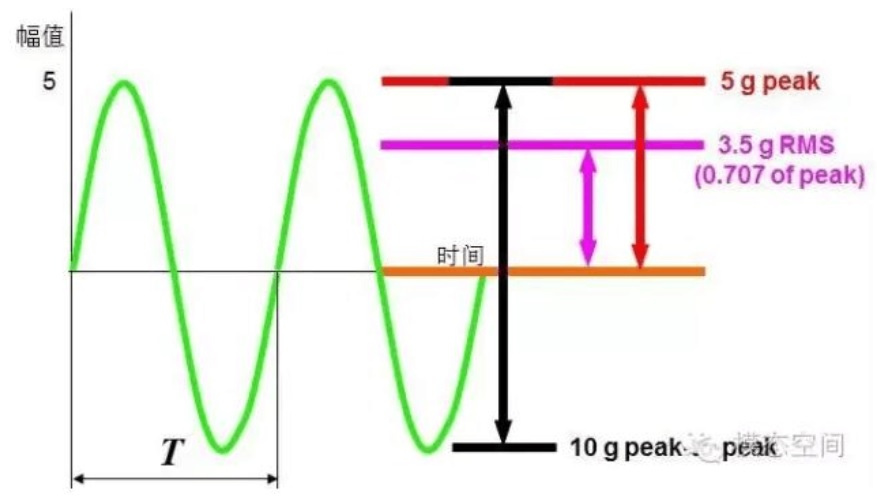
\includegraphics[height=7cm]{sin_wave.jpg}
		\caption{正弦波波形图}\label{正弦波波形图}
	\end{figure}
	可以看到Peak,RMS和Peak-Peak对应的关系如下表所示:
	\begin{table}[htbp] %htbp代表表格浮动位置
		%表格居中
		\centering
		%添加表头
		\caption{Peak,RMS和Peak-Peak}
		%创建table环境
		\begin{tabular}{ccc} %4个c代表4列都居中,也可以设置l,r
			%表格的输入
			\hline  %一条水平线
			Peak & RMS &Peak-Peak\\ %\\为换行符
			\hline
			A &0.707A &2A\\
			\hline
		\end{tabular}
	\end{table}
	\par 那么在各种谱函数中,到底用哪种格式来表示呢?答案是用哪种格式都可以,因为通过FFT变换之后,频域中的每一条谱线都是单频信号,因此,其Peak,RMS和Peak-Peak都是可以按上表中的关系式相互转换域中的每一条谱线都是单频信号,因此,其Peak,RMS和Peak-Peak都是可以按上表中的关系式相互的。一般商业软件默认的可能是Peak格式。某一个信号其自谱线性形式的这三种格式表示如下图\ref{RMS_PEAK_PP}所示,可以看出,这三条曲线是满足上表关系的。
	\begin{figure}[htbp]
		\centering
		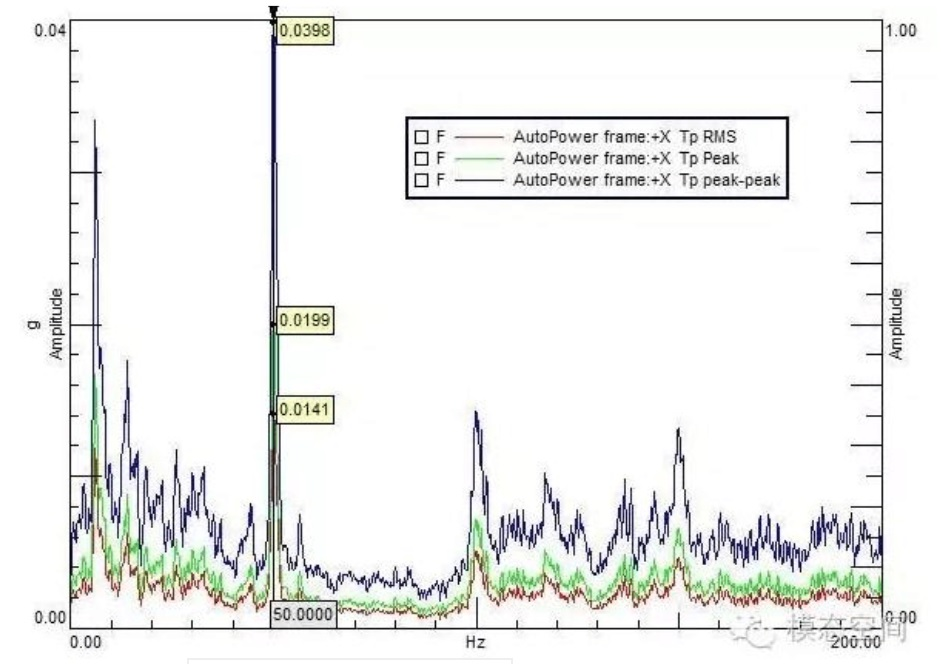
\includegraphics[height=7cm]{rms_peak_PP.jpg}
		\caption{RMS、PEAK、PP波形显示}\label{RMS_PEAK_PP}
    \end{figure}

	
	% 一般为了文章的分段清晰,采用空行来实现
	\section{Hilbert变换-Hilbert谱、Hilbert边际谱和包络谱}
	\subsection{Hilbert变换}
	一个实数值的希尔伯特变换(hilbert transform)H这里用 $\boldsymbol{H}$表示,将信号s(t)与$\frac{1}{\pi t}$	做卷积得到$\hat s(t)$,可以认为是s(t)的线性非时变系统的输出,而此一系统的脉冲响应为$\frac{1}{\pi t}$,希尔伯特转换是以著名数学家大卫·希尔伯特(David Hilbert)来命名。
	\begin{equation}
		\hat s(t)=\boldsymbol{H}(s)=h(t)*s(t)=\int_{-\infty}^{+\infty} {s(\tau)h(t-\tau)\mathrm{d}x}=\frac{1}{\pi}\int_{-\infty}^{+\infty}{\frac{s(\tau)}{t-\tau}\mathrm{d}x}
	\end{equation}
	其中
	\begin{equation}
		h(t)=\frac{1}{\pi t}
	\end{equation}
	
	Hilbert谱:信号的希尔伯特变换后做fft
	
	Hilbert边际谱:对hilbert谱做积分
	
	Hilbert包络谱:希尔伯特变换后做包络后再fft
	
	Hilbert谱表示的是信号幅值在整个频率段上随时间和频率的变化规律,Hilbert边际谱表示信号幅值在整个频率段上随频率的变化情况,它相当于傅里叶谱,但比傅里叶谱具有更高的频率分辨率。Hilbert边际谱是通过对Hilbert谱积分得到的。
	
	Hilbert包络谱不同于Hilbert谱和Hilbert边际谱,而是直接信号进行Hilbert变换后构造解析函数,然后依据解析函数求模值,求的模值即为包络,然后对信号包络进行FFT后得到的即为Hilbert包络谱。
	
	\section{为啥叫一阶线性系统}
	\begin{equation}
		\frac{\mathrm{d}y}{\mathrm{d}x}+ay(t)=bx(t)
	\end{equation}
	微分是指方程中包含导数,阶数是指方程中最高导数项的次数,线性是指输出y(t)的任何阶的导数项都是分开的,没有平方或多次方,也没有相乘,这是不是满足线性空间下的叠加性?,我暂且这么认为,满足的,所以叫做一阶线性微分方程。有不同意见可以和我探讨哈。
\end{document}